\section{古代计数方法}

\subsection{古埃及}

\begin{frame}\frametitle{古埃及}
	\begin{figure}\centering
		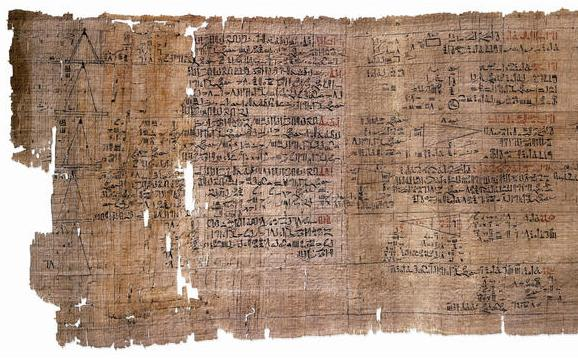
\includegraphics[width=0.8\textwidth]{Rhind_Mathematical_Papyrus.jpg}
		\caption{莱因德数学纸草书,著于约公元前1700年}
	\end{figure}
\end{frame}

\begin{frame}\frametitle{古埃及}
	\begin{block}{莱因德数学纸草书}
		总长525厘米、高33厘米,现藏大英博物馆。\\
		纸草书的内容分两部分:前面是一个分数表,后面是84个数学问题和一段无法理解的话(也称为问题85)。\\
		问题涉及素数、合数和完全数,算术,几何,调和平均数以及简单筛法等概念,其中还有对$\pi$的简单计算,所得值为3.1605。
	\end{block}
\end{frame}

\begin{frame}{古埃及}
	\begin{figure}\centering
		\subfigure{
			\includegraphics<1->[width=0.45\textwidth]{numbers1.jpg}
		}
		\subfigure{
			\includegraphics<2>[width=0.45\textwidth]{numexam21.jpg}
		}
	\caption{古埃及数字}
	\end{figure}
\end{frame}

\begin{frame}{古埃及}
\begin{exampleblock}{这是多少?}
	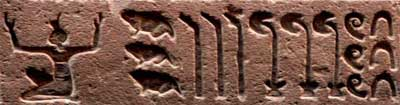
\includegraphics[width=0.8\textwidth]{numbers2.jpg}
\end{exampleblock}\pause
\begin{answer}
	1,333,330
\end{answer}
\end{frame}

\begin{frame}{古埃及}
	\begin{figure}\centering
		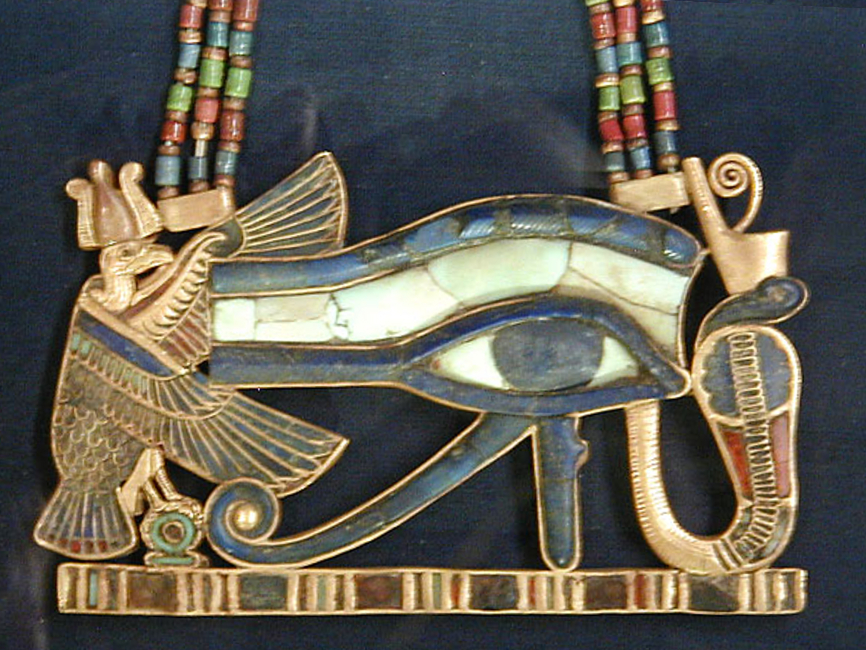
\includegraphics[width=0.45\textwidth]{Wedjat_(Udjat)_Eye_of_Horus_pendant.jpg}
		\caption{荷鲁斯之眼}
	\end{figure}
\end{frame}

\begin{frame}{古埃及}
	\begin{block}{荷鲁斯之眼}
		荷鲁斯之眼顾名思义,它是鹰头神荷鲁斯的眼睛。\\
		荷鲁斯的右眼象征完整无缺的太阳,依据传说,因荷鲁斯战胜赛特,右眼有著远离痛苦,战胜邪恶的力量。\\
		荷鲁斯的左眼象征有缺损的月亮,依据传说,荷鲁斯后来将左眼献给欧西里斯,因而左眼亦有分辨善恶、捍卫健康与幸福的作用,亦使古埃及人也相信荷鲁斯的左眼具有复活死者的力量。
	\end{block}
\end{frame}

\begin{frame}{古埃及}
	\begin{figure}\centering
		\subfigure{
			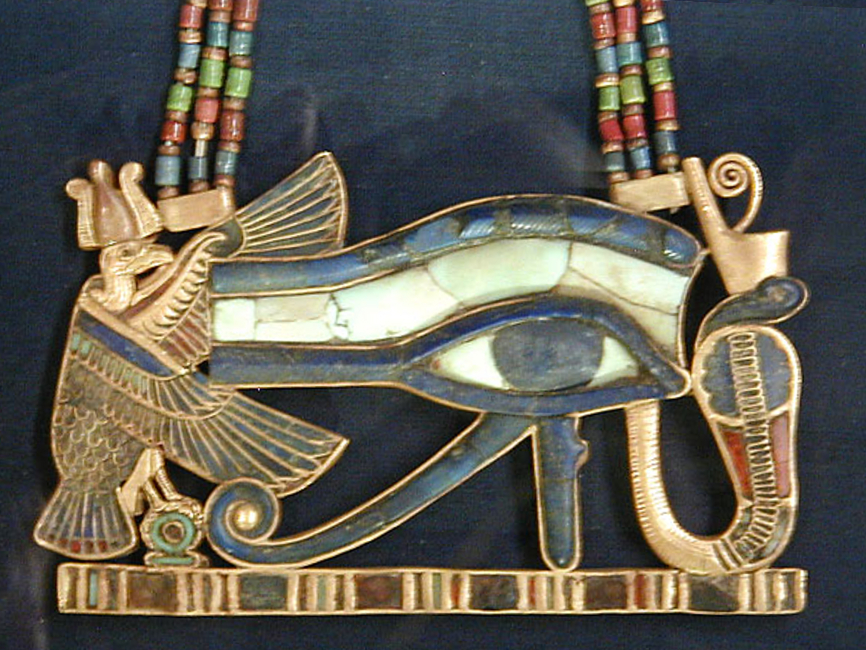
\includegraphics[width=0.45\textwidth]{Wedjat_(Udjat)_Eye_of_Horus_pendant.jpg}
		}
		\subfigure{
			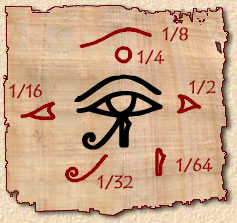
\includegraphics[width=0.47\textheight]{frac.jpg}
		}
		\caption{荷鲁斯之眼}
	\end{figure}
\end{frame}

\subsection{古巴比伦}

\begin{frame}\frametitle{古巴比伦}
	\begin{figure}\centering
		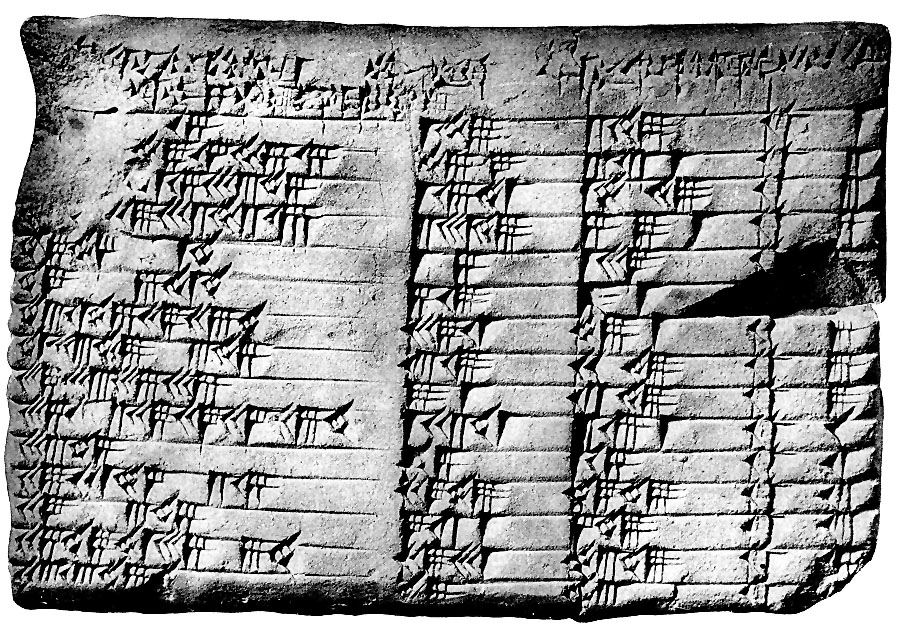
\includegraphics[width=0.8\textwidth]{Plimpton_322.jpg}
		\caption{普林顿322,刻于约公元前1800年}
	\end{figure}
\end{frame}

\begin{frame}\frametitle{古巴比伦}
	\begin{block}{普林顿322}
		普林顿 322为古巴比伦的一个泥板,约13厘米宽,9厘米高,2厘米厚,现藏于哥伦比亚大学。\\
		泥板上有一个四个行十五列和楔形文字组成的表格,表格列出了15组勾股数。
	\end{block}
\end{frame}

\begin{frame}\frametitle{古巴比伦}
	\begin{figure}\centering
		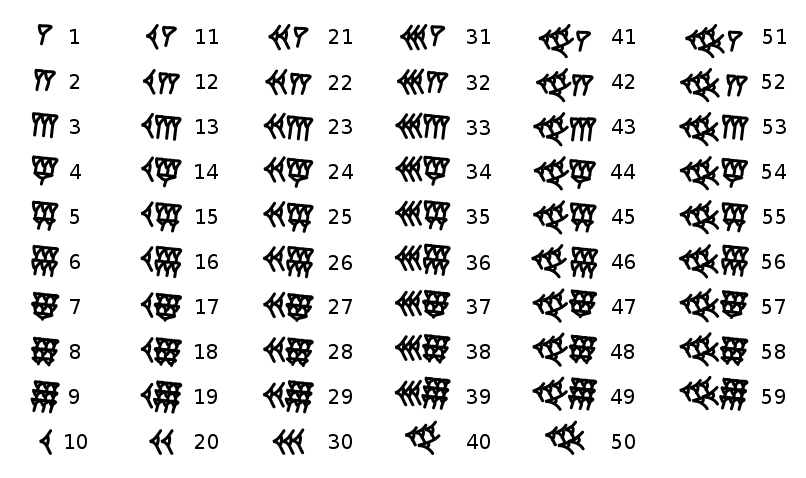
\includegraphics[height=0.5\textheight]{Babylonian_numerals.png}
		\caption{巴比伦数字}
	\end{figure}
\end{frame}

%\begin{frame}\frametitle{古巴比伦}
%	\begin{columns}[c]
%		\begin{column}{.5\textwidth}
%			\begin{figure}\centering
%				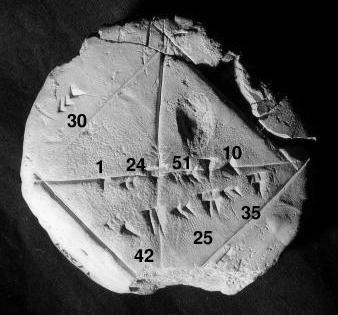
\includegraphics[width=.8\textwidth]{Ybc7289-bw.jpg}
%				\caption{巴比伦泥板 YBC 7289}
%			\end{figure}
%		\end{column}
%		\begin{column}{.5\textwidth}
%			对角线表示2的平方根,用4个六十进制的数字表示:
%			\[1+\dfrac{24}{60}+\dfrac{51}{60^2}+\dfrac{10}{60^3}=1.41421296...\]
%		\end{column}
%	\end{columns} 
%\end{frame}

\subsection{古印度}

\begin{frame}\frametitle{古印度}
	\begin{figure}\centering
		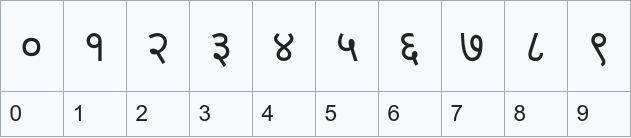
\includegraphics[width=0.8\textwidth]{Selection_110.png}
		\caption{天城文数字}
	\end{figure}
\end{frame}

\subsection{古中国}

\begin{frame}\frametitle{古中国}
	\begin{figure}\centering
		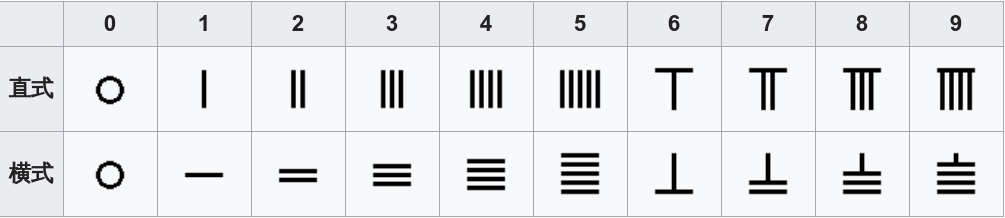
\includegraphics[width=0.5\textwidth]{Selection_111.png}
		\caption{算筹正数}
	\end{figure}\pause
	\begin{figure}\centering
		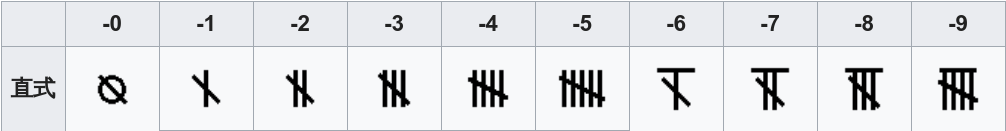
\includegraphics[width=0.5\textwidth]{Selection_112.png}
		\caption{负数}
	\end{figure}\pause
	\begin{figure}\centering
		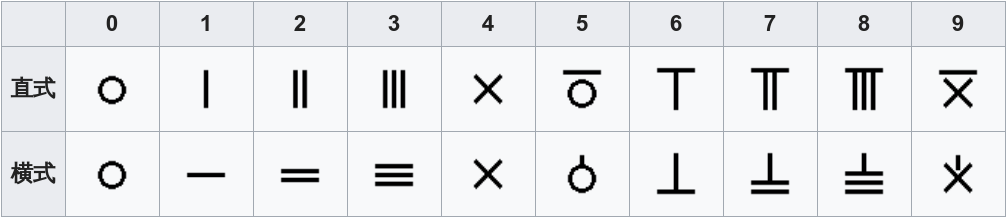
\includegraphics[width=0.5\textwidth]{Selection_113.png}
		\caption{南宋正筹码}
	\end{figure}
\end{frame}

\begin{frame}{古中国}
	\begin{figure}
		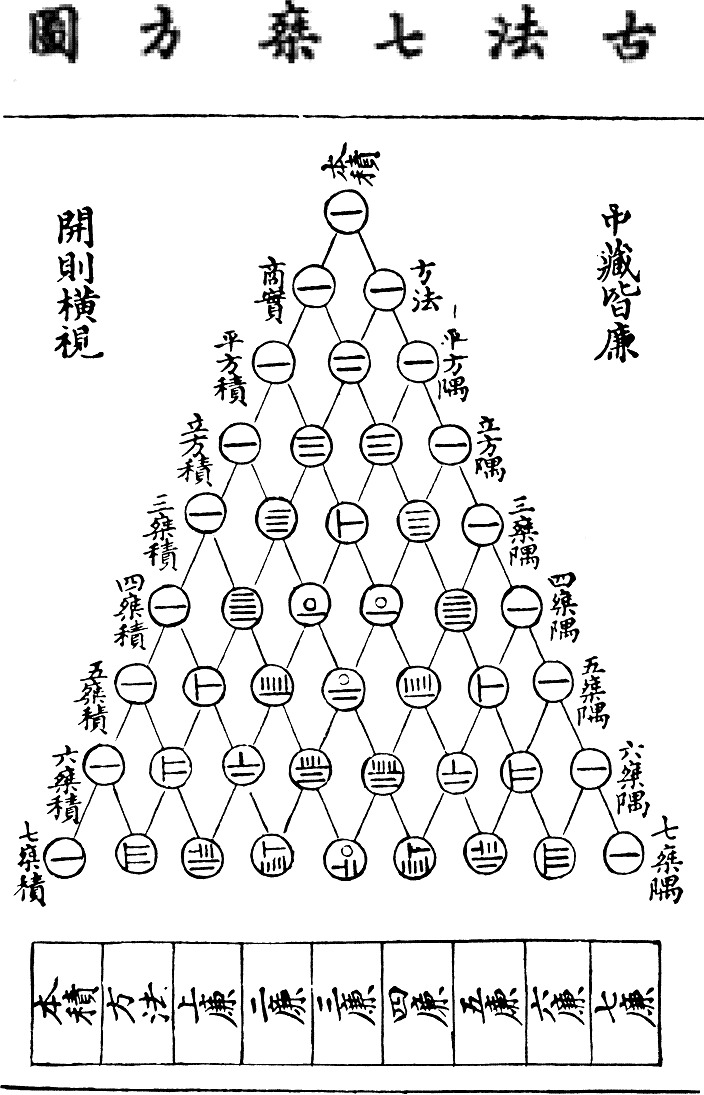
\includegraphics[height=0.7\textheight]{Yanghui_triangle.jpg}
		\caption{杨辉三角}
	\end{figure}
\end{frame}